
Previous work on large-scale collections of labels or names of objects has (explicitly or implicitly) assumed that once naming data is canonical, linguistic alternatives of the canonical name can simply be retrieved from existing taxonomies like e.g.\ WordNet. 
If this was indeed the case, it would be feasible (and probably even desirable) to canonicalize object names during dataset collection, without loosing too much information about linguistic variations in natural object naming scenarios (like e.g.\ referring expression generation).
Hence, in this section, we investigate to what extent the variation in object naming that we find in our MN data set (see previous Section) is covered by WordNet.

\subsection{Lexical relations}

In this section, we take a closer look at the lexical variation we observe in our data set. We analyze the data points where participants attributed different names to the same object and extract a set of  pairwise \textbf{naming variants}. These naming variants correspond to pairs of words that can be used interchangeably to name certain objects.
For each object, we extract the set of naming variants $s = \{ (w_{top},w_2), (w_{top},w_3), (w_{top},w_4),... \}$  where $w_{top}$ is the most frequent name annotated for the object and $w_2 ... w_n$ constitute the less frequent alternatives of $w_{top}$.  The  \textbf{type frequency} of a naming variant $(w_{top},w_x)$ corresponds to the number of objects where this variant occurs. The \textbf{token frequency} of $(w_{top},w_x)$ corresponds the count of all annotations where $w_x$ has been used instead of $w_{top}$.
In Table \ref{tab:exvariants}, we show the naming variants with the highest raw token frequency for each domain. 

The naming variants can be grouped according to their lexical relation, as follows:

\begin{itemize}
\item \textbf{synonymy}: e.g.\ aircraft vs. airplane 
\item \textbf{hyponymy}: e.g.\ man vs. person
\item \textbf{co-hyponymy}: e.g.\ swan vs. goose
\item \textbf{no relation}: e.g.\  desk vs. apple
\end{itemize}

\begin{table}
\small
\centering
\begin{tabular}{lcc}
\toprule
         relation & \% types & \% token \\
\midrule
 meronym &  0.1 &  0.2 \\
 holonym &  0.1 &  0.4 \\
 synonym &  1.1 &  1.1 \\
 hyponym &  2.2 &  3.8 \\
 co-hyponym &  3.1 &  5.9 \\
 hypernym &  10.5 &  27.7 \\
 word-not-covered &  10.6 &  2.6 \\
 rel-not-covered &  72.2 &  58.3 \\
\bottomrule
\end{tabular}

%\begin{tabular}{lll}
%\toprule
%       relation &  types & tokens \\
%\midrule
%synonymy &  0.01 &  0.09 \\
%co-hyponymy &  0.03 &  0.07 \\
%hypernymy &  0.06 &  0.35 \\
%not-covered &  0.19 &  0.04 \\
%crossclassified &  0.70 &  0.47 \\
%\bottomrule
%\end{tabular}
% \small
% \begin{tabular}{llll}
% \toprule
%         relation & \% types & \% tokens & av. depth \\
% \midrule
%  co-hyponymy (closure, max depth=10) &  0.889 &  0.551 &       3.479 \\
%     hyponymy (closure, max depth=10) &  0.097 &  0.328 &       2.204 \\
%         synonymy &  0.015 &  0.121 &       1.000 \\
% \bottomrule
% \end{tabular}

%\begin{tabular}{l|ll|ll|ll|ll|ll}
%\toprule
%      & \multicolumn{2}{c}{crossclassified} & \multicolumn{2}{c}{co-hyponymy} & \multicolumn{2}{c}{hypernymy} & \multicolumn{2}{c}{not-covered} & \multicolumn{2}{c}{synonymy} \\
%         domain & typ & tok & typ & tok & typ & tok & typ &  tok & typ & tok \\
%\midrule
% people &  0.725 &  0.618 &  0.019 &  0.032 &  0.051 &  0.293 &  0.200 &  0.038 &  0.005 &  0.019 \\
% clothing &  0.709 &  0.661 &  0.020 &  0.046 &  0.045 &  0.195 &  0.219 &  0.085 &  0.008 &  0.012 \\
% animals\_plants &  0.679 &  0.461 &  0.032 &  0.102 &  0.111 &  0.365 &  0.167 &  0.058 &  0.011 &  0.014 \\
% food &  0.590 &  0.433 &  0.031 &  0.033 &  0.104 &  0.432 &  0.267 &  0.089 &  0.009 &  0.013 \\
% vehicles &  0.635 &  0.329 &  0.026 &  0.083 &  0.059 &  0.239 &  0.271 &  0.089 &  0.008 &  0.260 \\
% home &  0.672 &  0.644 &  0.026 &  0.072 &  0.040 &  0.130 &  0.254 &  0.097 &  0.009 &  0.057 \\
% buildings &  0.780 &  0.725 &  0.026 &  0.038 &  0.045 &  0.156 &  0.138 &  0.058 &  0.011 &  0.022 \\
% \hline
% all &  0.731 &  0.574 &  0.033 &  0.057 &  0.076 &  0.256 &  0.147 &  0.050 &  0.013 &  0.064 \\
%\bottomrule
%\end{tabular}


\caption{Lexical relations of naming variants in MN to annotated VG synset, averaged over synsets}
\label{tab:rel}
\end{table}


Research on object naming following the idea of entry-level categories has, essentially, exclusively looked at names that stand in a hierarchical relation (i.e.\ hyponymy/hypernymy).

We use WordNet to extract lexical relations between the naming variants in our data set.
Unfortunately, this means that we have to exclude a certain portion of the data as either (i) one of the name is not covered in WordNet, (ii) we cannot find a lexical relation between the two names (see below). Also, we had to be relatively permissive with respect to the definition of hyponymy/co-hyponymy. 
For instance, to analyze \textit{giraffe} as a hyponym of \textit{animal} we have to look at the closure of the hyponyms of \textit{animal} with a depth of 8 (in WordNet).
\sz{should we call this co-hyponymy or co-hierarchical relation?}

\sz{include Table that reports counts of the naming variants, coverage in WordNet etc.} \gbt{I think it'd be best to put the out-of-wordnet info in the Lexical relations table -- this way we have everything in one place.}

Table \ref{tab:rel} shows the distribution of lexical relations for those naming variants that we were able to analyze with WordNet.
Both in terms of their types and token frequency, the naming variants that instantiate a (loose) co-hyponymy relation are by far the most frequent.
\sz{discuss in more detail, discuss: to what extent is this an artefact of WordNet?}
This is really interesting: most research on object naming, to date, has focussed on hyponymy/hypernymy, i.e. variation that relates to hierarchical relations between object names.
Our data suggests that co-hierarchical variation is really important too.

\subsection{The ``no relation'' case}

For each domain, we manually annotated the 100 most frequent name pairs in the ``no relation'' case. Table~\ref{tab:crossclass} shows that, in this category, one third of the pairs do refer to the same object, but the relationship is not captured in WordNet. 
Most of these cases are arguably coverage issues of WordNet, which doesn't capture the co-hyponymy of \textit{horse}-\textit{donkey} or the fact that \textit{vehicle} is hypernym of \textit{train}.\gbt{I find this really weird... also some other cases I annotated. It sounds like I should have listened more carefully to Carina when she suggested going down and up in the wordnet hierarchy (cf.\ the example of food-fruit). :/ Maybe we'd capture quite a bit of them if we did a more sophisticated querying of WordNet. To discuss.}
% between \textit{hat}-\textit{beanie}.
However, a substantial group is constituted by names whose denotations overlap even if they don't belong to the same category. These are typically alternative conceptualizations of objects: as a cat or a toy, as a kind of building or its function (\textit{building}-\textit{home}), or as a portion or a kind of food (\textit{pizza-slice}).

Still, 69\% of the annotated pairs arguably do not denote the same object. Here we find problems HUMANS MAKE SAME ``ERRORS'' AS MACHINES -- REFERENTIAL UNCERTAINTY IN THE ABSENCE OF CONTEXT (discuss as planned with Carina).


Interesting name pairs:

\begin{itemize}
\item storefront - store: strictly speaking it's part-whole, but how can one distinguish between the two? 
\item field - grass: same (reverse); how to distinguish?
\item dog - pet (different conceptualizations; classified as ``hypernym.2'')
\item airplane - flight, plane - flight (classified as ``other'').
\end{itemize}


Most of the cases are co-hyponyms with categories that are easily confused, such as \textit{horse}-\textit{donkey}, \textit{truck}-\textit{jeep}.
In some cases, the visual cues are not enough to distinguish between the categories, but the frequency of this phenomenon suggests that co-hyponyms can be used interchangeably.


\begin{figure*}
\begin{minipage}[b]{0.5\linewidth}
{\footnotesize
\setlength{\tabcolsep}{1pt}
\begin{tabular}{cp{4cm}p{4cm}p{4cm}}
\textbf{desk} &  \raisebox{-\totalheight}{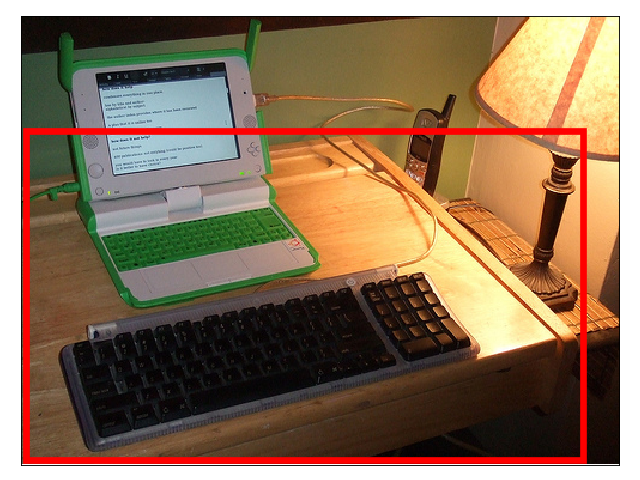
\includegraphics[width=0.9\linewidth]{figures/2320949_1048853_singleton_obj.png}} MN: keyboard  &
\raisebox{-\totalheight}{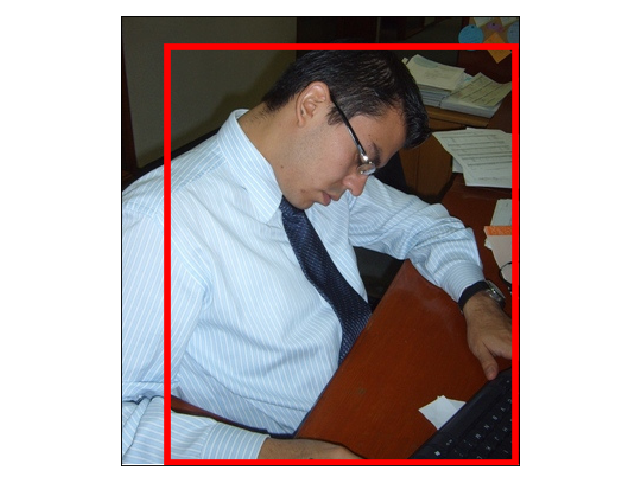
\includegraphics[width=0.9\linewidth]{figures/2343219_926143_supercat_unique.png}}  MN: desktop &
\raisebox{-\totalheight}{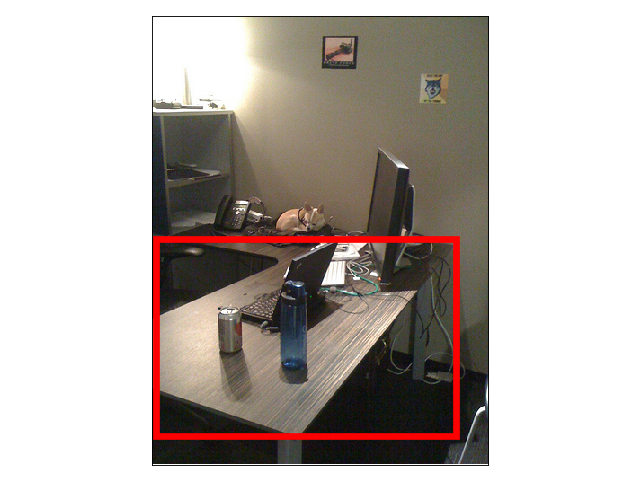
\includegraphics[width=0.9\linewidth]{figures/2354847_1742687_seed_ambiguous.png}} MN: computer \\
\textbf{bench} &  \raisebox{-\totalheight}{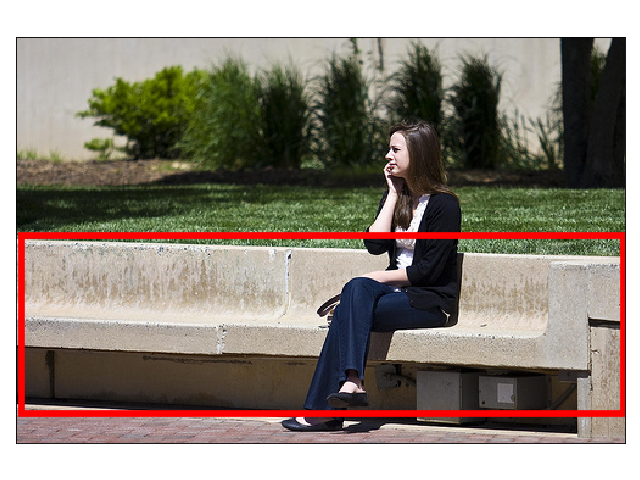
\includegraphics[width=0.9\linewidth]{figures/2350360_1042111_supercat_unique.png}} MN: table  &
\raisebox{-\totalheight}{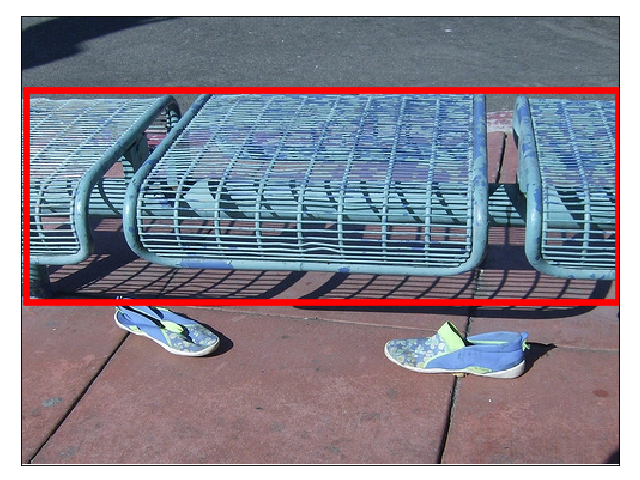
\includegraphics[width=0.9\linewidth]{figures/2389358_1261752_singleton_obj.png}}  MN: seat &
\raisebox{-\totalheight}{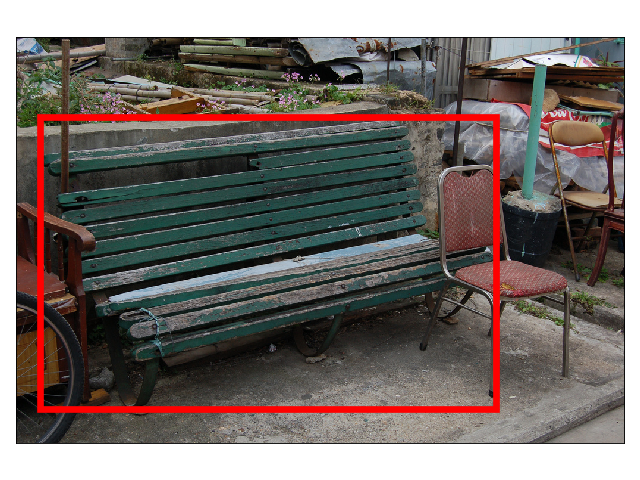
\includegraphics[width=0.9\linewidth]{figures/1593011_2063521_singleton_obj.png}} MN: wood \\
\textbf{sandwich} &  \raisebox{-\totalheight}{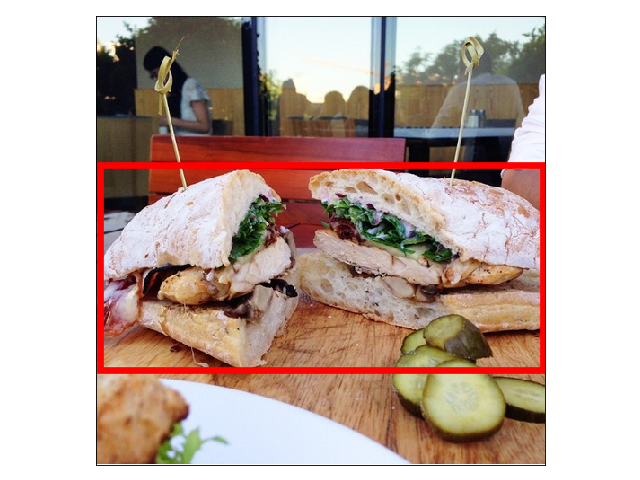
\includegraphics[width=0.9\linewidth]{figures/2352086_856151_supercat_unique.png}} MN: burger  &
\raisebox{-\totalheight}{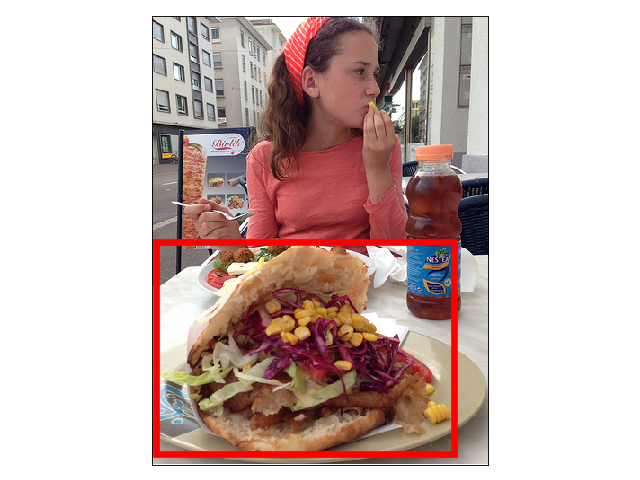
\includegraphics[width=0.9\linewidth]{figures/2352833_1884120_supercat_unique.png}}  MN: plate &
\raisebox{-\totalheight}{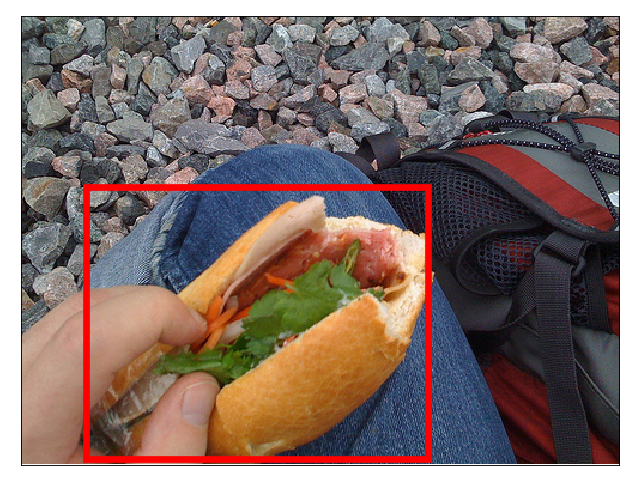
\includegraphics[width=0.9\linewidth]{figures/2343230_2309969_supercat_unique.png}} MN: bun\\ 
\textbf{girl} &  \raisebox{-\totalheight}{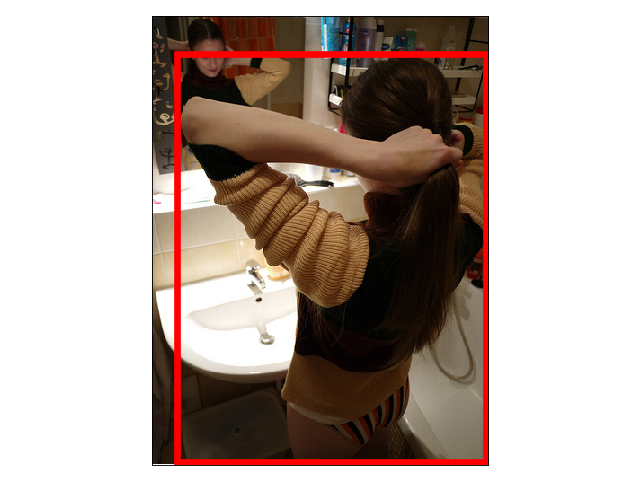
\includegraphics[width=0.9\linewidth]{figures/2400735_406112_singleton_obj.png}} MN: t-shirt  &
\raisebox{-\totalheight}{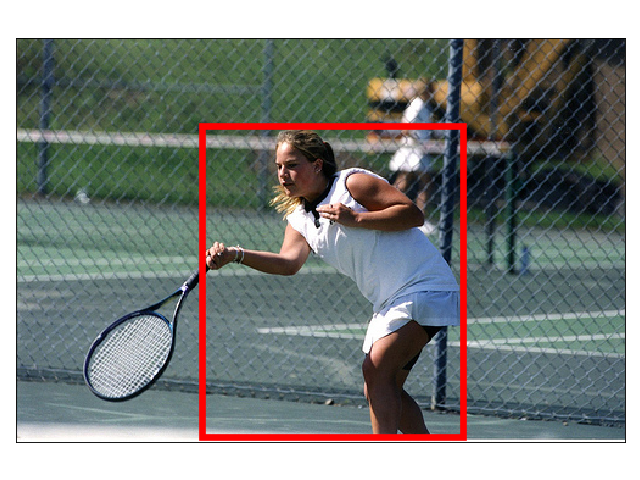
\includegraphics[width=0.9\linewidth]{figures/2329628_3363001_singleton_obj.png}}  MN: tennis player &
\raisebox{-\totalheight}{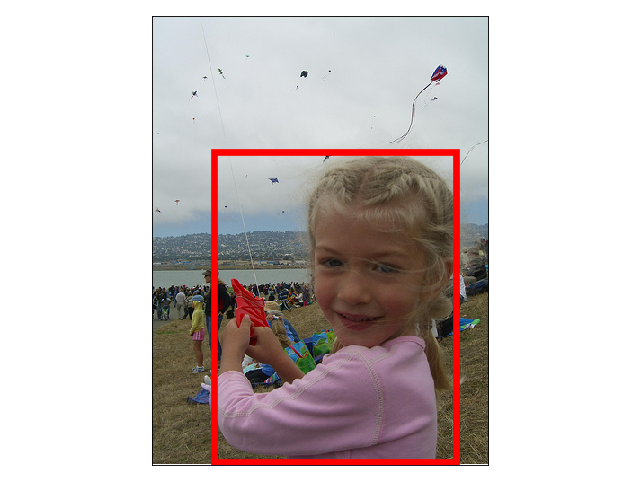
\includegraphics[width=0.9\linewidth]{figures/2315383_1055824_singleton_obj.png}} MN: kid\\ 
\textbf{truck} &  \raisebox{-\totalheight}{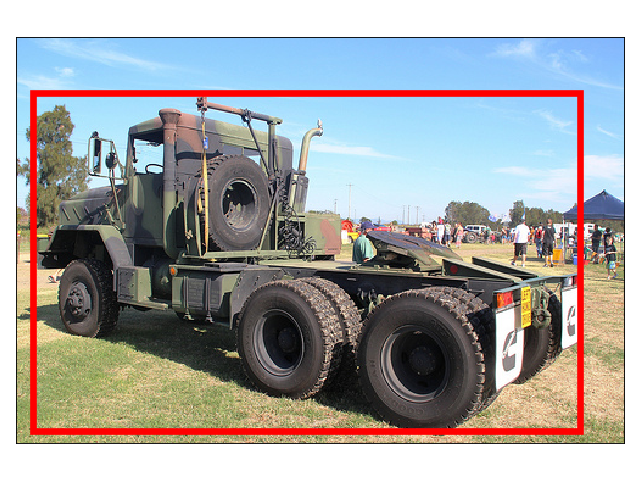
\includegraphics[width=0.9\linewidth]{figures/2317240_1022463_singleton_obj.png}} MN: wheel  &
\raisebox{-\totalheight}{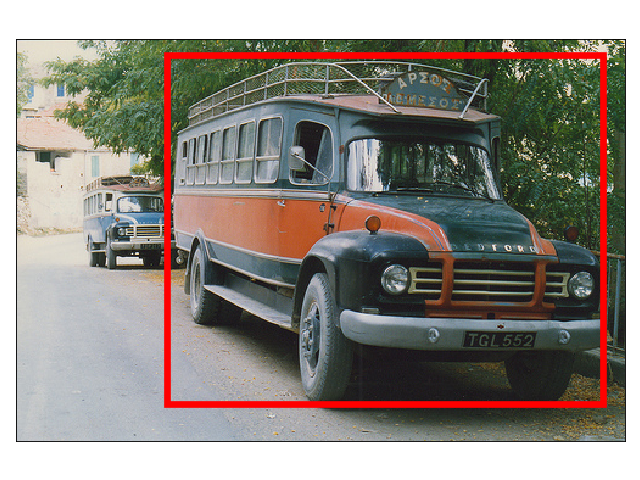
\includegraphics[width=0.9\linewidth]{figures/2410889_361670_singleton_obj.png}}  MN: bus &
\raisebox{-\totalheight}{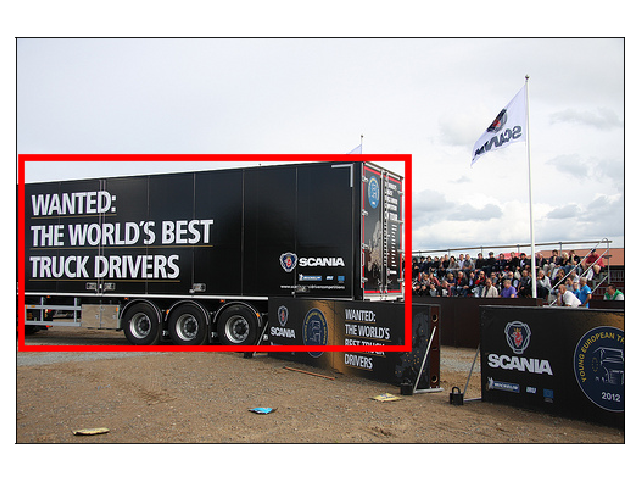
\includegraphics[width=0.9\linewidth]{figures/2334129_965945_singleton_obj.png}} MN: trailer\\ 
\textbf{bridge} &  \raisebox{-\totalheight}{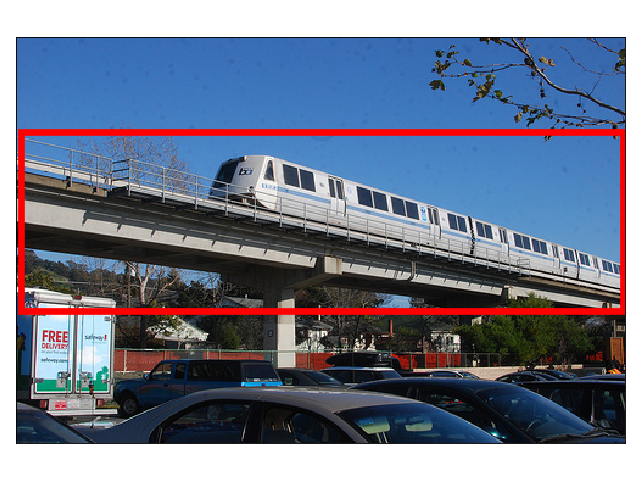
\includegraphics[width=0.9\linewidth]{figures/2349701_3192266_supercat_unique.png}} MN: train  &
\raisebox{-\totalheight}{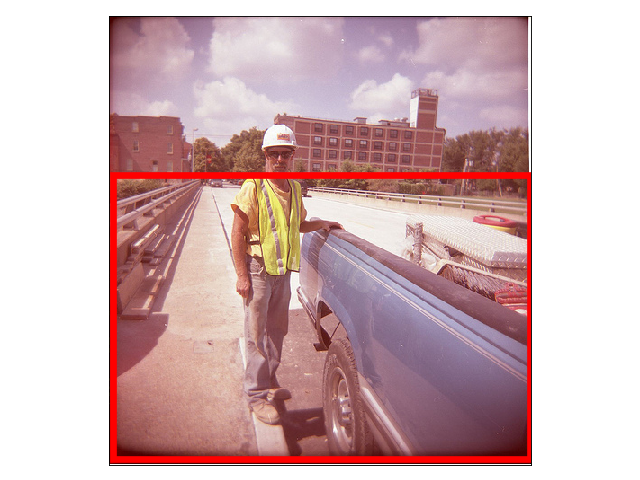
\includegraphics[width=0.9\linewidth]{figures/2322428_2930306_supercat_unique.png}}  MN: road &
\raisebox{-\totalheight}{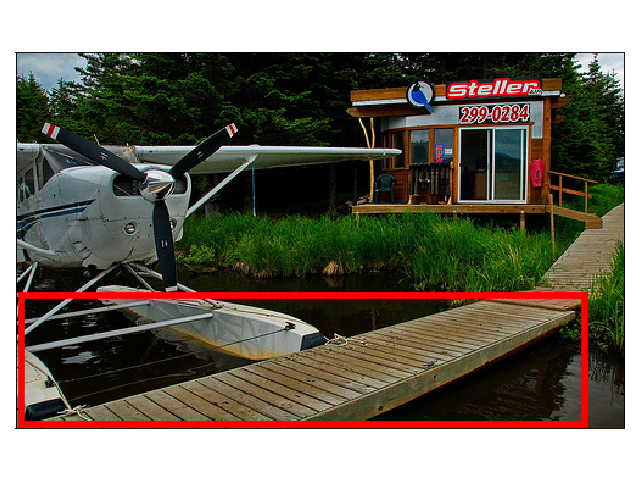
\includegraphics[width=0.9\linewidth]{figures/2348679_2628081_supercat_unique.png}} MN: dock\\ 
\textbf{bed} &  \raisebox{-\totalheight}{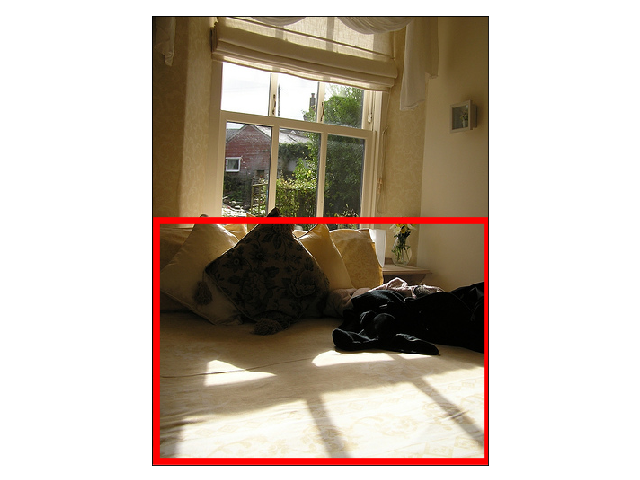
\includegraphics[width=0.9\linewidth]{figures/2400919_1153609_singleton_obj.png}} MN: pillow  &
\raisebox{-\totalheight}{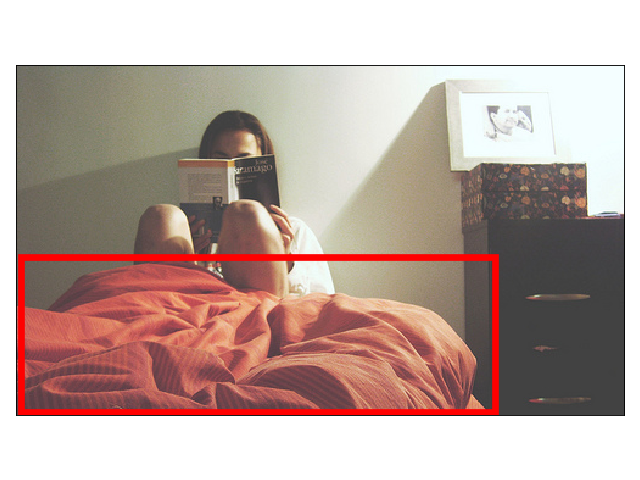
\includegraphics[width=0.9\linewidth]{figures/2383991_529114_singleton_obj.png}}  MN: blanket &
\raisebox{-\totalheight}{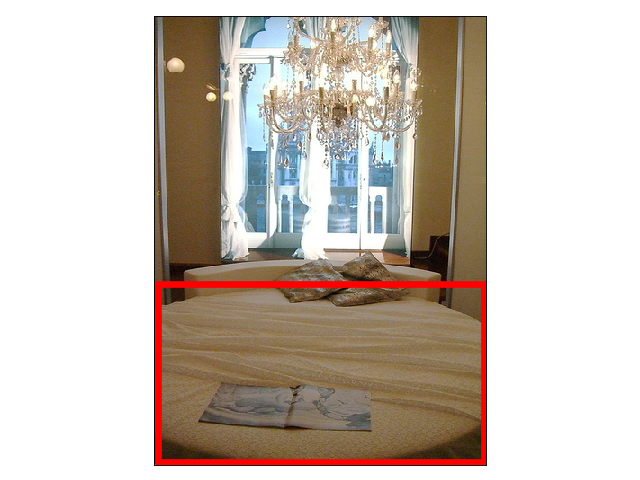
\includegraphics[width=0.9\linewidth]{figures/2343909_918810_singleton_obj.png}} MN: table\\ 

\end{tabular}

}
\end{minipage}

 \caption{\label{fig:ex}Examples from MN data set, where no relation between VG synset (in bold) and name annotation can be found}
\end{figure*}


